%%%%%%%%%%%%%%%%%%%%%%%%%%%%%%%%%%%%%%%%%
% Journal Article
% LaTeX Template
% Version 1.3 (9/9/13)
%
% This template has been downloaded from:
% http://www.LaTeXTemplates.com
%
% Original author:
% Frits Wenneker (http://www.howtotex.com)
%
% License:
% CC BY-NC-SA 3.0 (http://creativecommons.org/licenses/by-nc-sa/3.0/)
%
%%%%%%%%%%%%%%%%%%%%%%%%%%%%%%%%%%%%%%%%%

%----------------------------------------------------------------------------------------
%	PACKAGES AND OTHER DOCUMENT CONFIGURATIONS
%----------------------------------------------------------------------------------------

\documentclass[twoside]{article}

\usepackage{graphicx}
\usepackage{lipsum} % Package to generate dummy text throughout this template

\usepackage[sc]{mathpazo} % Use the Palatino font
\usepackage[T1]{fontenc} % Use 8-bit encoding that has 256 glyphs
\linespread{1.05} % Line spacing - Palatino needs more space between lines
\usepackage{microtype} % Slightly tweak font spacing for aesthetics

\usepackage[hmarginratio=1:1,top=32mm,columnsep=20pt]{geometry} % Document margins
\usepackage{multicol} % Used for the two-column layout of the document
\usepackage[hang, small,labelfont=bf,up,textfont=it,up]{caption} % Custom captions under/above floats in tables or figures
\usepackage{booktabs} % Horizontal rules in tables
\usepackage{float} % Required for tables and figures in the multi-column environment - they need to be placed in specific locations with the [H] (e.g. \begin{table}[H])
\usepackage{hyperref} % For hyperlinks in the PDF

\usepackage{lettrine} % The lettrine is the first enlarged letter at the beginning of the text
\usepackage{paralist} % Used for the compactitem environment which makes bullet points with less space between them
\usepackage{amsmath}
\usepackage{abstract} % Allows abstract customization
\renewcommand{\abstractnamefont}{\normalfont\bfseries} % Set the "Abstract" text to bold
\renewcommand{\abstracttextfont}{\normalfont\small\itshape} % Set the abstract itself to small italic text

\usepackage{titlesec} % Allows customization of titles
\renewcommand\thesection{\Roman{section}} % Roman numerals for the sections
\renewcommand\thesubsection{\Roman{subsection}} % Roman numerals for subsections
\titleformat{\section}[block]{\large\scshape\centering}{\thesection.}{1em}{} % Change the look of the section titles
\titleformat{\subsection}[block]{\large}{\thesubsection.}{1em}{} % Change the look of the section titles

\usepackage{fancyhdr} % Headers and footers
\pagestyle{fancy} % All pages have headers and footers
\fancyhead{} % Blank out the default header
\fancyfoot{} % Blank out the default footer
\fancyhead[C]{PHSX567 Final Project Proposal $\bullet$ \today } % Custom header text
\fancyfoot[RO,LE]{\thepage} % Custom footer text


%----------------------------------------------------------------------------------------
%	TITLE SECTION
%----------------------------------------------------------------------------------------

\title{\vspace{-15mm}\fontsize{24pt}{10pt}\selectfont\textbf{MOSES Data Inversion With Convolutional Neural Networks}} % Article title

\author{
\large
\textsc{Roy Smart}\\[2mm] % Your name
\normalsize Montana State University \\ % Your institution
\normalsize \href{mailto:roytsmart@gmail.com}{roytsmart@gmail.com} % Your email address
\vspace{-5mm}
}
\date{}

%----------------------------------------------------------------------------------------

\begin{document}

\maketitle % Insert title

\thispagestyle{fancy} % All pages have headers and footers



%----------------------------------------------------------------------------------------
%	ARTICLE CONTENTS
%----------------------------------------------------------------------------------------

\begin{multicols}{2} % Two-column layout throughout the main article text

\section{Introduction}
The Multi-Order Solar EUV Spectrograph (MOSES) is a unique instrument that captures solar images in three diffraction orders: $m=0,+1,$ and $-1$. Unlike most spectrographs, MOSES is not equipped with a slit to restrict the field of view in the direction of dispersion. This advantage of this configuration is that spectral and spatial information is simultaneously viewed by the instrument, allowing interesting solar features to be more easily identified. However this lack of spatial restriction by a slit means that spectral and spatial information are convolved together to form the images captured by MOSES. These images are known as "overlappograms." \par
\begin{figure}[H]
	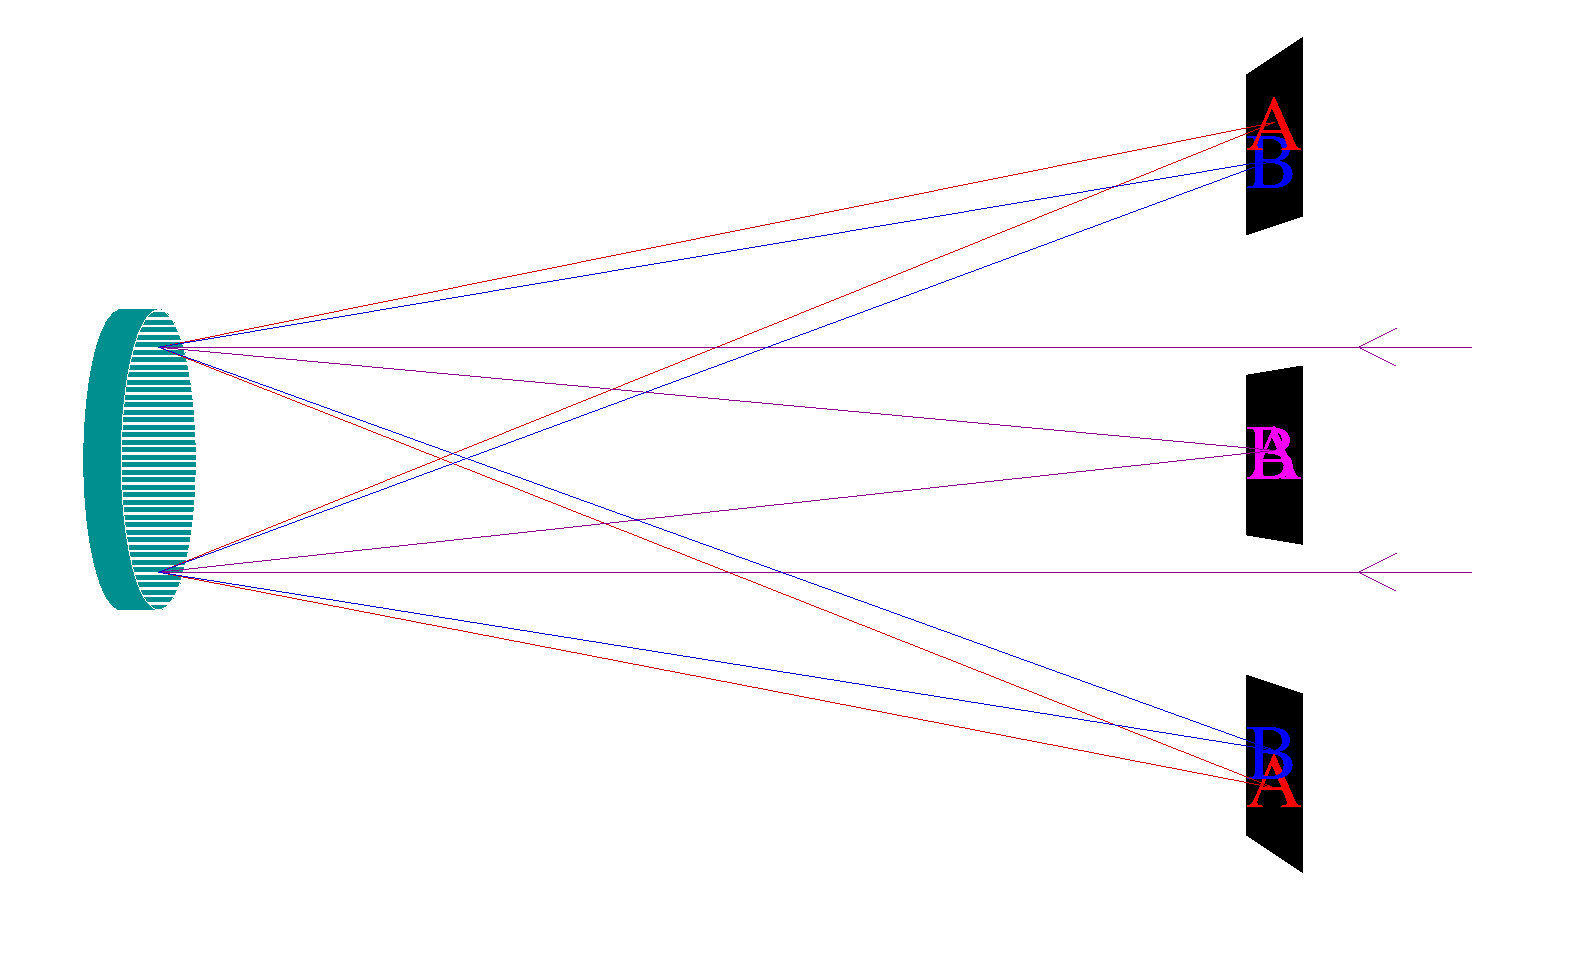
\includegraphics[width=\linewidth]{images/instrument.eps}
	\caption{Layout of the MOSES instrument demonstrating how different wavelengths are overlapped onto each detector.}
\end{figure}
The main objective of the MOSES instrument is to determine Doppler shifts of the structures observed in the solar transition region. To find this quantity, we must perform what we call an \textit{inversion}. This is best described as taking the 2-dimensional spectral and spatial information from each of the three detectors and constructing a spectral \textit{cube} in three dimensions, with two spatial dimensions and one spectral dimension.
\begin{figure}[H]
	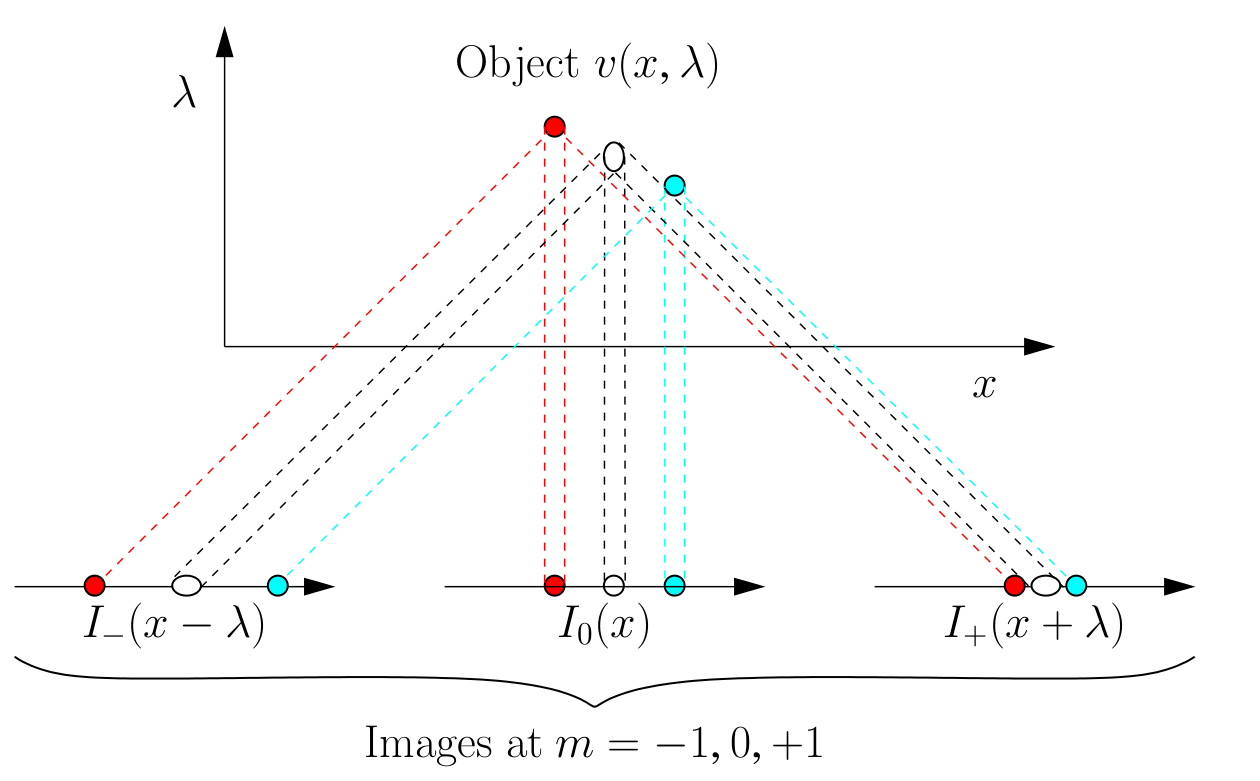
\includegraphics[width=\linewidth]{images/inversion}
	\caption{Diagram demonstrating how compact objects in the data cube are convolved to form the images at each detector \cite{moses}.}
\end{figure}
The main challenge with inverting the MOSES data is that it is an obviously ill-posed problem, i.e. the spectral cube contains more information than is provided by the instrument. This is mathematically described using the expression
\begin{equation}
I_m(x',y') = \int_B v(x'-m \lambda,y',\lambda)d\lambda \label{invert}
\end{equation}
Where $I(x',y')$ is the intensity measured by the instrument $v(x',y',\lambda)$ is an object located in the spectral cube, $m$ is the spectral order, $(x',y')$ are the detector coordinates, and the domain $B$ is the passband of the instrument. 
\par Since Equation \eqref{invert} doesn't have a unique solution, there are many possible cubes that could produce the same images captured by MOSES. The task then, is to try and use what we know about physics to try and trim down the large number of potential data cubes in an attempt to learn something about the solar transition region. \par 

\section{Motivation}

Many researchers over the history of the MOSES research project have developed computational tools to solve the inversion problem. These methods are discussed in detail in the literature and include Smoothed Multiplicative Algebraic Reconstruction Technique (SMART)\cite{smart}, Fourier backprojection and pixon inversion \cite{inversion}. 
\par These methods are very powerful and they have proved successful in revealing the interior structure of the transition region \cite{moses}. However there is still room for progress to be made towards full inversions of the entire MOSES dataset. These algorithms have a tendency to produce what is known as \textit{plaid}. This is where bright objects on the spectral cube tend to be smeared across the direction of the spectral projections, producing decidedly unphysical inversions.

\begin{figure}[H]
	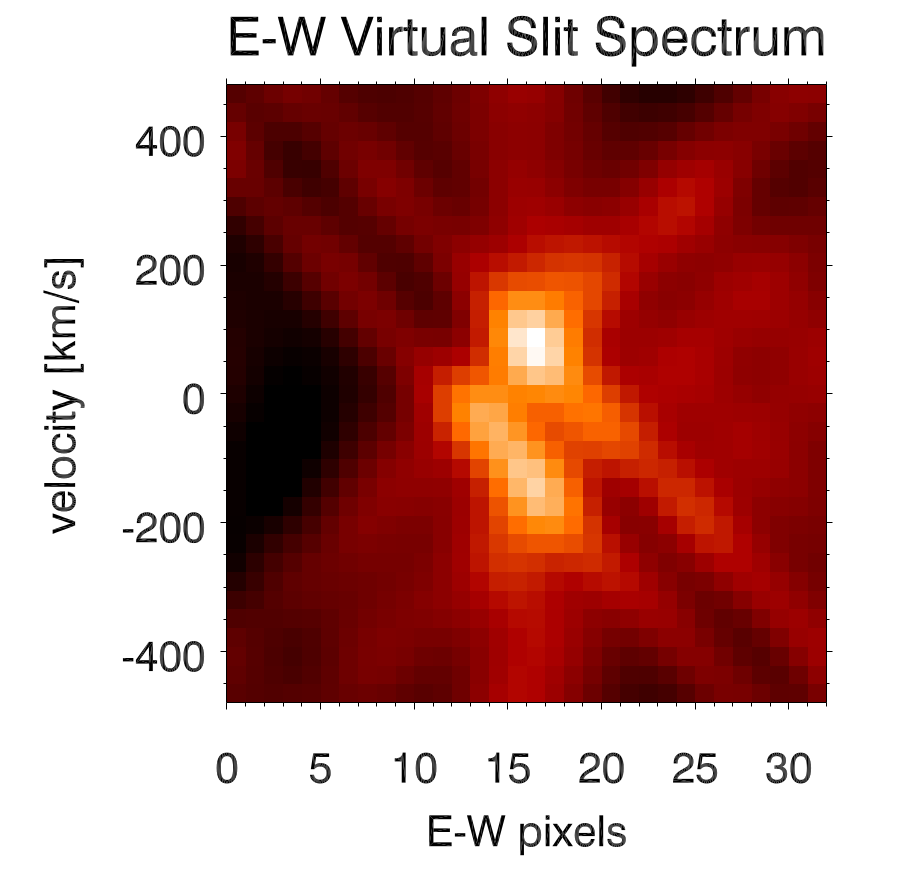
\includegraphics[width=\linewidth]{images/plaid2}
	\caption{An example of plaid. Notice how the bright pixels in the center are smeared diagonally across the image. This is an example of an unphysical inversion. \cite{tom} }
\end{figure} 

Determining an inversion method that is resistant to plaid would be very beneficial to Kankelborg's research group, as inversions would contain valuable scientific data.

\section{Proposed Inversion Method}
\subsection{Machine Learning}
Thus far, all of the attempts to invert the MOSES data have relied on traditional, human-designed algorithms to carry out the computation. However, in the past few years, great strides have been made in machine learning, where a computer program is presented with a problem and its solution and then \textit{trained} to solve the problem using a large number of  problem/solution examples. \par I propose that a method based off of machine learning might allow some progress to be made towards the goal of plaid-resistant MOSES inversions. This is made possible by the fact that the learning algorithm could be penalized for producing plaid solutions to the inversion problem and rewarded for producing physical solutions.  \par While all this machine learning sounds fantastic, there is still a great deal of challenges to contend with. First, the structure of the learning algorithm is very important, and unlike traditional algorithms, the right structure can often only be found by trial and error. Furthermore, the learning process takes a large number of examples to converge on the solution. Solving these problems will be discussed in the following pages.

\subsection{Artificial Neural Networks}

Artificial neural networks (ANNs) are machine learning algorithms that are modeled off of the structure of the human brain. ANNs can be described as a system of \textit{neurons} that have the ability to communicate with each other. The behavior of each neuron is dictated by an activation function. This function maps neuron inputs to outputs, e.g. determines when the neuron is \textit{active}. Active neurons propagate information through the network while dormant neurons restrict it.  \par Communication is facilitated through a series of connections between the neuron, where each connection may have a different weight representing the amount of influence one neuron may have on another. The weights are tuned based off of experience and taken with the activation function, allow the neural network to learn. \par The neurons are usually organized into layers, where each layer can be interpreted as a different computational step used to solve the problem. The first layer is known as the input layer, and the number of input neurons corresponds to the amount of information supplied to the network. The output layer is the last layer, and the number of output neurons equals the amount of information to be expected in the solution of the problem being solved. In between the input and output layers, there is a number of hidden layers used to compute the solution. The amount of hidden layers and the number of neurons per hidden layer depends on the complexity of the problem.
\begin{figure}[H]
	\centering
	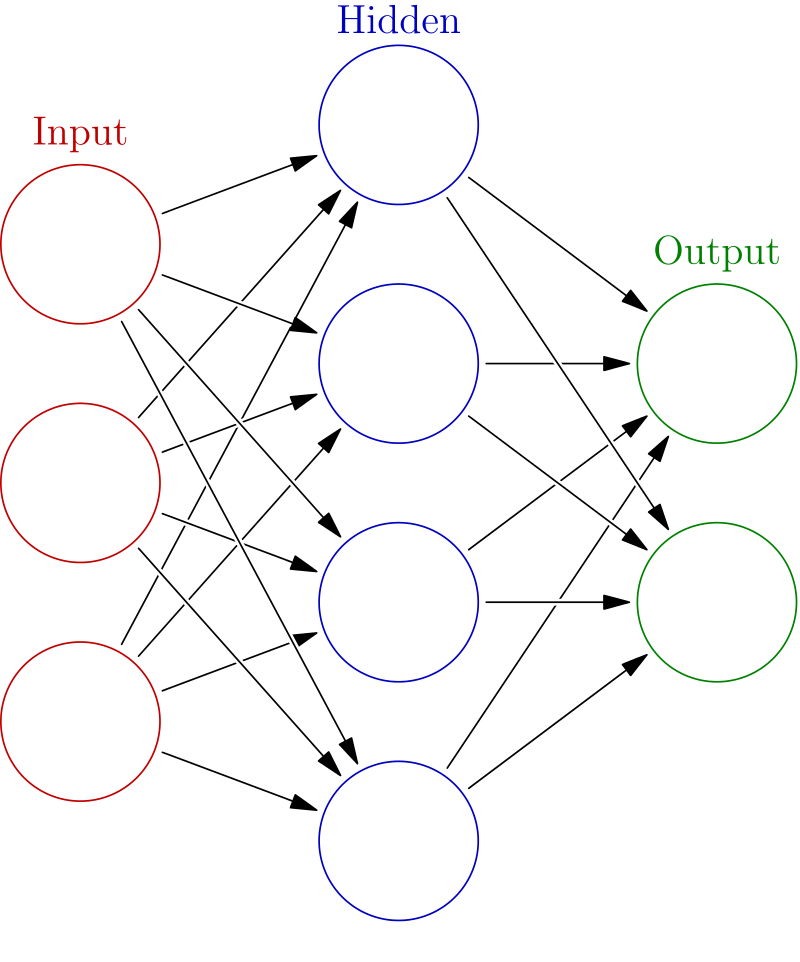
\includegraphics[width=0.5\linewidth]{images/neural}
	\caption{An example of a simple neural network.}
\end{figure}
Using this simple idea, many different species of neural networks may be constructed. The choices of network depth, number of connections, and activation function are examples of what are called \textit{hyperparameters}, and determine the behavior of the network.

\subsection{Convolutional Neural Networks}
Vanilla ANNs usually connect each neuron in one layer to every other neuron in the preceding layer. This configuration is sufficient when the number of input neurons is small. However, when the number of input neurons grows as large as an image, for example, the huge number of free parameters quickly leads to overfitting. Furthermore, the Vanilla ANN treats pixels with large spatial separation equally, which is often undesirable for image processing where close spatial relationships are more important. \par Convolutional Neural Networks (CNNs) solve this problem by connecting only a small number of the input neurons (known as the receptive field) to the layers below, known as convolutional layers.
\begin{figure}[H]
	\centering
	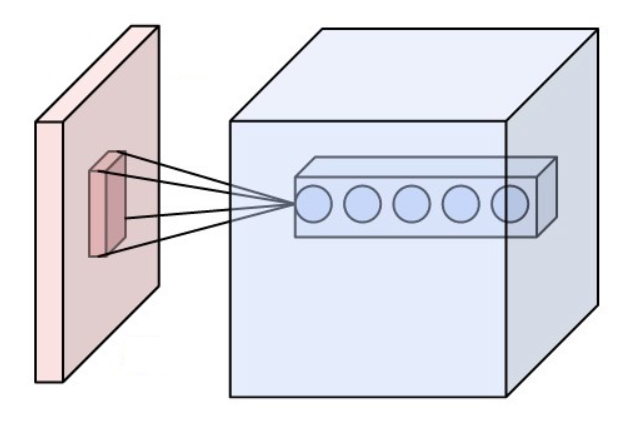
\includegraphics[width=0.5\linewidth]{images/Conv_layer}
	\caption{The red box represents the input neurons, with the receptive field connected to the next five convolutional layers.}
\end{figure}
The receptive fields are tiled such that they overlap one another. Overlapping receptive fields, taken with parameter sharing with the convolutional layers in the network provides translational invariance and amounts to a convolution operation (hence the name). There are many other layers that go into a CNN that will not be discussed here, but they include: pooling, RELU, and fully connected layers. These layers serve to increase the computational power and decrease the training time of the network. \par CNNs have been used successfully in many fields, most notably in image recognition \cite{imagenet}. We think that this type of neural network will be best suited to MOSES data inversion because spectral features in MOSES images are separated spatially, and CNNs are optimized to detect spatial features in images.

\section{Implementation}
\subsection{Selecting Hyperparameters}
We are not yet sure how best to select the hyperparameters for the network. Most networks in the literature consist of approximately five convolutional layers, one or more pooling layers, one or more RELU layers, and one fully connected layer. Determining the topography of the network is one of the major challenges that lies ahead.
\subsection{Training Dataset}
The training dataset needs to contain the data gathered by MOSES and the spectral cube that produced the result. Since we do not yet know the answer to the MOSES inversion problem, we will need to look to other sources to provide the data. An obvious choice is the data collected by the IRIS satellite. IRIS is a traditional slit spectrograph, and thus has independent dimensions for spectral and spatial data. The idea then, is to use the information collected by IRIS to simulate MOSES data. IRIS has a collected a large dataset during its mission, so there should be plenty of training data to tune the CNN.
\subsection{Hardware}
Training large, interesting neural networks has only recently become tractable for personal computers. While CPUs have only been demonstrating modest floating-point performance gains over the past few years, GPUs have been following an exponential trend. Furthermore, GPUs are designed with massive parallelism in mind, which can be utilized by a neural network algorithm. Therefore, it is advantageous to take advantage of current GPU performance to quickly train neural networks. 

\subsection{Software}
Developing such an advanced neural network would take quite a lot of time, especially for a GPU implementation. Luckily enough, one has already been developed for us. \textit{Caffe} is a convolutional neural network program, developed at Berkley for image processing \cite{caffe}. \par Caffe allows the user to define their network as a simple script, and then trains the network on an Nvidia GPU automatically. Once the network is trained it may be run on either a CPU or GPU. This will prove useful as we can guarantee that the network will still be usable, regardless of hardware developed in the near future.

\end{multicols}

	\bibliographystyle{unsrt}
	\bibliography{sources}
\end{document}
